\documentclass{article}

\usepackage{graphicx}
\usepackage{float}
\graphicspath{ {./images/} }

\title{Scalar Spherical Harmonics and Slepian Functions}
\author{}
\date{}


\setlength{\parskip}{0.5cm plus4mm minus3mm}

\textwidth=6.4in
\textheight=8.5in
\hoffset=-0.7in
\voffset=-0.7in

\setlength{\parindent}{0cm} 


\begin{document}
\maketitle

\tableofcontents 

\section{Plot a single spherical harmonic function}

We will demonstrate plotting a spherical-harmonic on a sphere,  in a standard Matlab plot, on a Mollweide projection, and on random points of a sphere.

First, designate a spherical-harmonic to be plotted:

For example,

\verb+l+ = 3; \verb+m+ = -2;

0 ≤ \verb+l+ fixes the degree and \verb+m+ fixes the order.

\subsection{Plot on sphere}

\setlength{\parskip}{.1mm}

\verb+l+ = 3; \verb+m+ = -2;

\verb+lon = 0:0.5:360;+

\verb+lat = -90:0.5:90;+

\verb+Y = ylm(l, m, pi/180*(90-lat), pi/180*lon);+

\verb+figure;+

\verb+plotplm(Y, pi/180*lon, pi/180*lat,2)+

\begin{figure}[H]
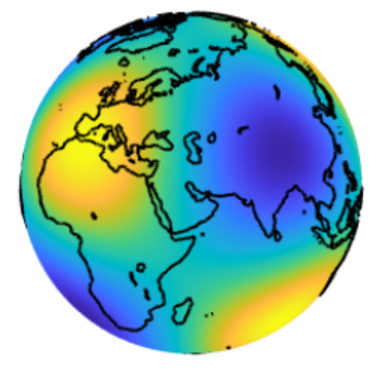
\includegraphics[scale=1]{graph_on_sphere}
\end{figure}

\setlength{\parskip}{0.5cm plus4mm minus3mm}

1. Create a grid on the sphere

\verb+lon = 0:0.5:360;+
\verb+lat = -90:0.5:90;+

This creates a coordinate point every half-degree.

2. Calculate the values of the function for coordinate points on the sphere

\verb+Y = ylm(l, m, pi/180*(90-lat), pi/180*lon);+

The function \verb+slepian_alpha/ylm.m+ evaluates the spherical harmonic function of degree \verb+l+ and order \verb+m+ at every point \verb+pi/180*(90-lat)+, \verb+pi/180*lon+ on the grid. We name the vector of the spherical-harmonic values “\verb+Y+”.

Note that \verb+90-lat+ is needed to convert latitude to colatitude and \verb+pi/180+ is needed to convert degrees to radians.

3. Plot

\verb+figure;+
\verb+plotplm(Y, pi/180*lon, pi/180*lat,2)+

The function \verb+slepian_alpha/plotplm.m+ is here used to plot the vector \verb+Y+ using the grid specified by “\verb+lon+” and “\verb+lat+” in step 1. The input \verb+2+ dictates that the graph be on a sphere.

\subsection{Plot in standard Matlab plot}

\setlength{\parskip}{.1mm}

\verb+l+ = 3; \verb+m+ = -2;

\verb+lon = 0:0.5:360;+

\verb+lat = -90:0.5:90;+

\verb+Y = ylm(l, m, pi/180*(90-lat), pi/180*lon);+

\verb+imagesc(lon, lat, Y)+

\begin{figure}[H]
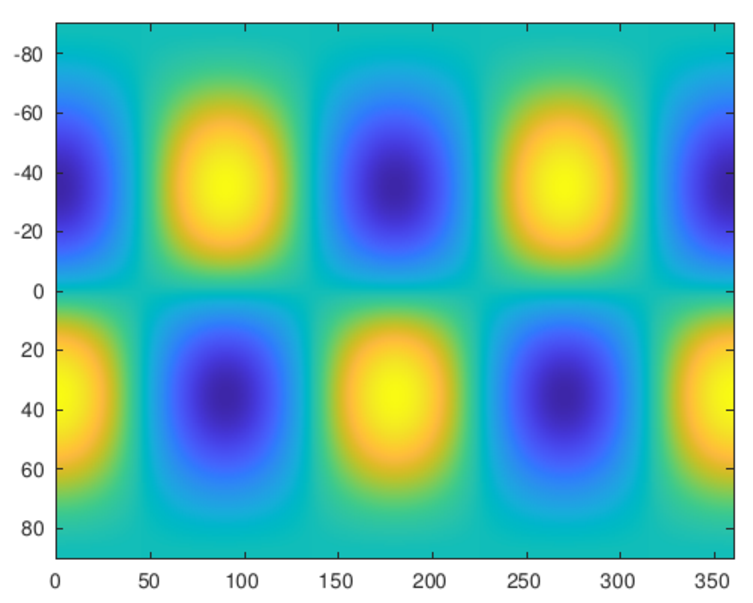
\includegraphics[scale=.6]{standard_matlab_plot}
\end{figure}

\setlength{\parskip}{0.5cm plus4mm minus3mm}

Do steps 1 and 2, and then run

\verb+imagesc(lon, lat, Y)+

\subsection{Plot on Mollweide projection}

\setlength{\parskip}{.1mm}

\verb+l+ = 3; \verb+m+ = -2;

\verb+lon = 0:0.5:360;+

\verb+lat = -90:0.5:90;+

\verb+Y = ylm(l, m, pi/180*(90-lat), pi/180*lon);+

\verb+figure;+

\verb+plotplm(Y, pi/180*lon, pi/180*lat,1)+

\begin{figure}[H]
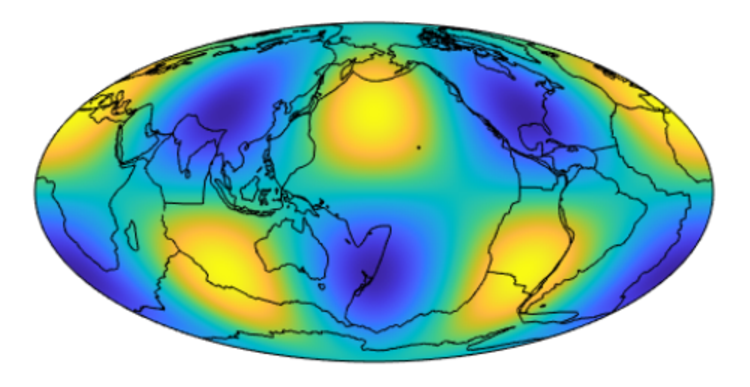
\includegraphics[scale=.8]{mollweide}
\end{figure}

\setlength{\parskip}{0.5cm plus4mm minus3mm}

Do steps 1 and 2, and then run

\verb+figure;+

\verb+plotplm(Y, pi/180*lon, pi/180*lat,1)+

The input \verb+1+ dictates that the graph be on the Mollweide projection.

\subsection{Plot for random points on a sphere}

\setlength{\parskip}{.1mm}

\verb+l+ = 3; \verb+m+ = -2;

\verb+TH = 120; lon0 = 30; cola0 = 40; N=1000;+

\verb+[lon, lat] = randpatch(N,TH,lon0,cola0);+

\verb+Y = ylm(l, m, pi/180*(90-lat), pi/180*lon,[],[],[],1);+

\verb+scatter(lon, lat, [], Y)+

\begin{figure}[H]
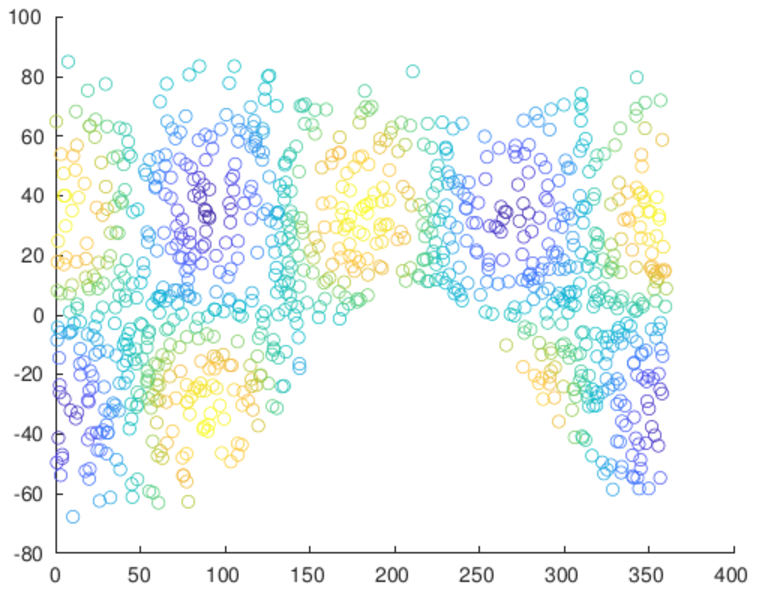
\includegraphics[scale=.75]{random_plot}
\end{figure}

\setlength{\parskip}{0.5cm plus4mm minus3mm}

1. Generate a subset of the sphere consisting of random points 

In particular, we will create \verb+N+ randomly-generated coordinate points within a spherical cap of opening angle \verb+TH+ and centered at longitude \verb+lon0+ and colatitude \verb+cola0+

For example, 

\verb+TH = 120; lon0 = 30; cola0 = 40; N=1000;+

\verb+[lon, lat] = randpatch(N,TH,lon0,cola0);+

The function \verb+slepian_alpha/randpatch.m+ creates the set of random points within the spherical cap of the specified values. We name those coordinate points \verb+[lon,lat]+.

2. Calculate the values of the spherical harmonic at those points

\verb+Y = ylm(l, m, pi/180*(90-lat), pi/180*lon,[],[],[],1);+


\verb+ylm.m+ takes the arguments \verb+l+, \verb+m+, \verb+pi/180*(90-lat)+, \verb+pi/180*lon+ as before. Run \verb+help ylm+ for information on all eight arguments. 

3. Plot

If necessary, use the Matlab command 

\verb+ clf;+

To clear existing figures, and then run the Matlab command

\verb+scatter(lon, lat, [], Y)+

To create a scatter plot of circles having locations \verb+[lon, lat]+. Here, \verb+[]+ indicates the default value for circle size and the vector of spherical-harmonic values \verb+Y+ is used to determine circle color. 

Please see \verb+Ch_01+ in the \verb+.edu+ folder for more detailed information.

\section{Plot a linear combination of spherical harmonics}

\setlength{\parskip}{.1mm}

\verb+lon = 0:0.5:360;+

\verb+lat = -90:0.5:90;+

\verb+Y1=ylm(3,1,pi/180*(90-lat),pi/180*lon);+

\verb+Y2=ylm(1,-1,pi/180*(90-lat),pi/180*lon);+

\verb+Y3=ylm(5,-2,pi/180*(90-lat),pi/180*lon);+

\verb!Y4=4*Y1-0.2*Y2+2*Y3;!

\verb+plotplm(Y4, pi/180*lon, pi/180*lat,1);+

\verb!kelicol(1)!
\begin{figure}[H]
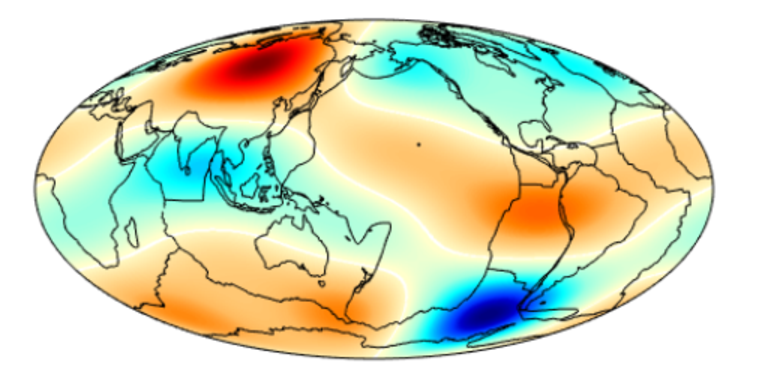
\includegraphics[scale=1]{linear_combination}
\end{figure}

\setlength{\parskip}{0.5cm plus4mm minus3mm}

This task is a simple variation on the first. 

Let us define three spherical harmonics:

\verb+lon = 0:0.5:360;+

\verb+lat = -90:0.5:90;+

\verb+Y1=ylm(3,1,pi/180*(90-lat),pi/180*lon);+

\verb+Y2=ylm(1,-1,pi/180*(90-lat),pi/180*lon);+

\verb+Y3=ylm(5,-2,pi/180*(90-lat),pi/180*lon);+

Next, create a vector which is a linear combination of these three. For example,

\verb!Y4=4*Y1-0.2*Y2+2*Y3;!

To plot the function, use \verb+plotplm.m+. For example,

\verb+plotplm(Y4, pi/180*lon, pi/180*lat,1)+

If you're interested in another color scheme, try out 

\verb+kelicol(1)+

Please see \verb+Ch_01+ in the \verb+.edu+ folder for more detailed information.

\end{document}